\section{Content Impact}

One aim of this research is to analyze the impact of new content posted by an influencer on their followers count.

To reach this purpose, has been downloaded all videos posted by an influencers over the past five months. For each video, has been registered the users who followed the influencer within five days after the video was posted.

\begin{lstlisting}[language=json]
{
    "data": {
        "cursor": 1717588518,
        "has_more": true,
        "user_followers": [
            {
                "username": "rev6luv",
                "display_name": "t."
            },
            {
                "display_name": "Caden M. Flanagan",
                "username": "therealcadenflanagan"
            },
            ...
    }
} 
\end{lstlisting}

There is a potential bias in this approach, as new followers can be gained independently of new posts. However, on social networks today, content either goes viral almost immediately or not at all. For this reason this approach has been considered valid.

The query included in the body of the request contains simply the username, without filtering other parameters (such as hashtag, region or anything else). This decision has been made since an influencer can talks about various topics but still is belongs to a specific wing. 

\begin{lstlisting}[language=json]
{
    "and": [
        {
            "operation": "IN",
            "field_name": "username",
            "field_values": [
                "$influencer" 
            ]
        }
    ]
}
\end{lstlisting}

For this analysis, has been considered just some influencer as considered the most influential (with more followers and engagement)

Monitoring the simple increasing of new followers through time, as can be seen, is slowly incrementing for almost all influencer.

Has been done a more specific analysis on two interesting influencer: "aocinthehouse" and "real.benshapiro".

\begin{figure}[h]
    \centering
    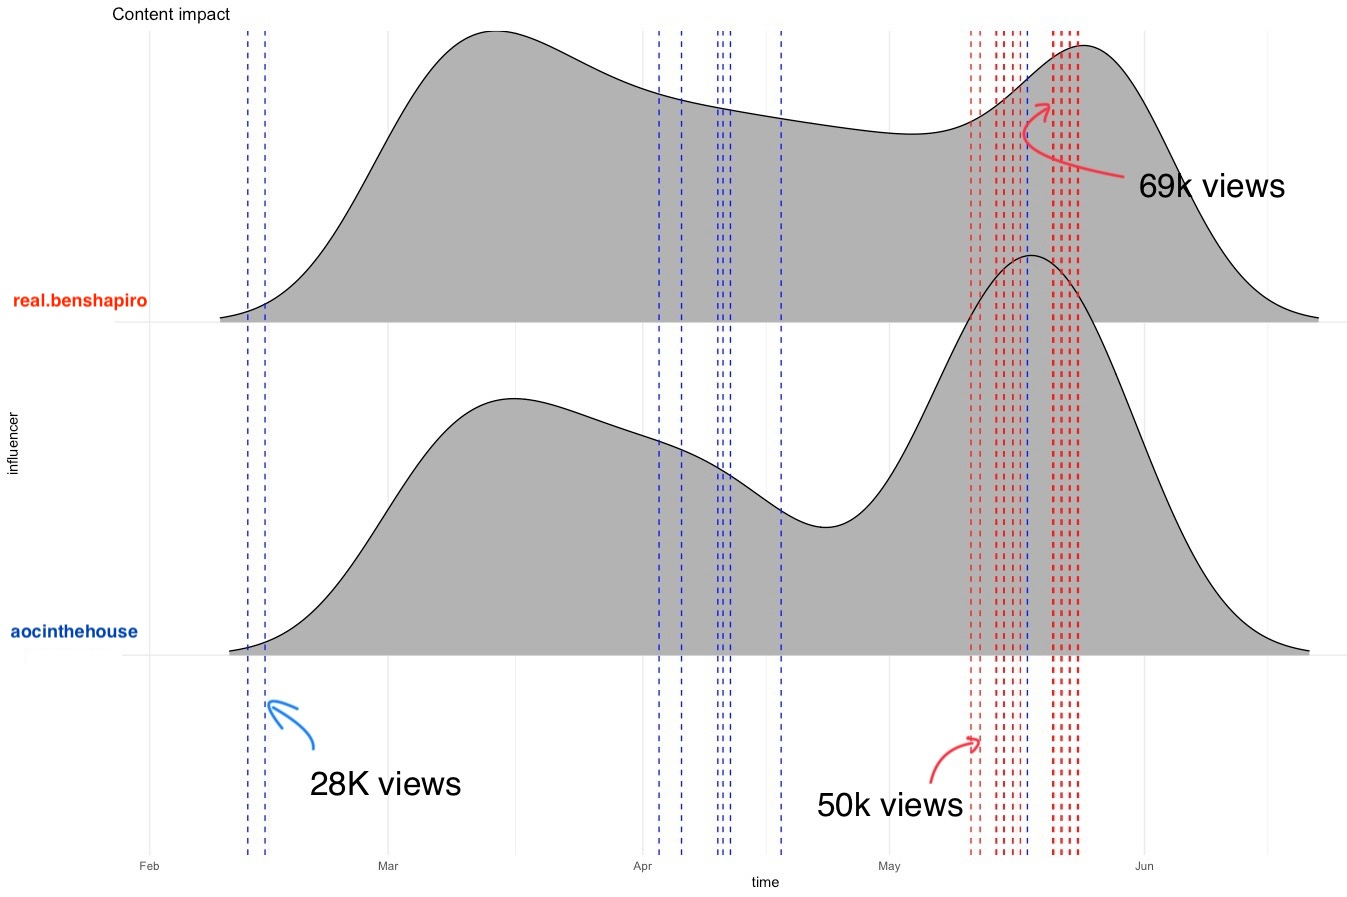
\includegraphics[width = .5\textwidth]{images/Final_ContentImpact_Custom.jpg}
    \caption*{This analysis consisted in the average trend of new followers, creating so a detailed curve enriched with timestamps of new post creations.}
\end{figure}

In example, there is a noticeable increase of new followers for "aocinthehoue" after the content posted on data 15 February with 28k.

Instead a curious fact is for "real.benshapiro" posting a lot of video with a low time gap but still gaining a increment without posting (on middle march), anyway this can confirm the bias assumed which the followers aren't just gained through tiktok platform. In fact, for example the official account of ben shapiro on 9th march 2024 has released a video with almost 300k views on YouTube (talking about political situation in Russia): \url{https://www.youtube.com/watch?v=GNye8kCfh4Y}.